\subsection{Overview}

The Robocup Logistic League is a competition to simulate Industry 4.0.  The goal of this contest is to use autonomous robots to fulfill some action by interacting with some industrial stations (MPS). Some constraints are applied like a defined number of MPSs, a defined size of field, a limited amount of time for each phase of the game. 

\subsection{Changes in 2017}

The Smartbots team has participate to Robocup German Open 2017 Magdeburg, Logistics League from 5. to 7. Mai 2017. Each year a new Rulebook is edited. This year, it was published one month before the German Open. The changes of the year 2017 was first a bigger field (14m x 8m) in comparison with last year (12m x 6m). There were also more zones and each zone was smaller (1m x 1m) in comparison with last year (2m x 1.5m). The number of MPS per team increased from 6 to 7 MPS with a new storage station. Before possible zones with a MPS was sent by the Refbox to each team at the beginning of the exploration phase. In the rules 2017, there are no information sent. It is now needed to explore the field and search for the 7 MPS and sent back to the Refbox the name of the MPS read with the help of the tag, the zone of MPS and the orientation of MPS. 

\begin{figure}%[tbhp]
\centering
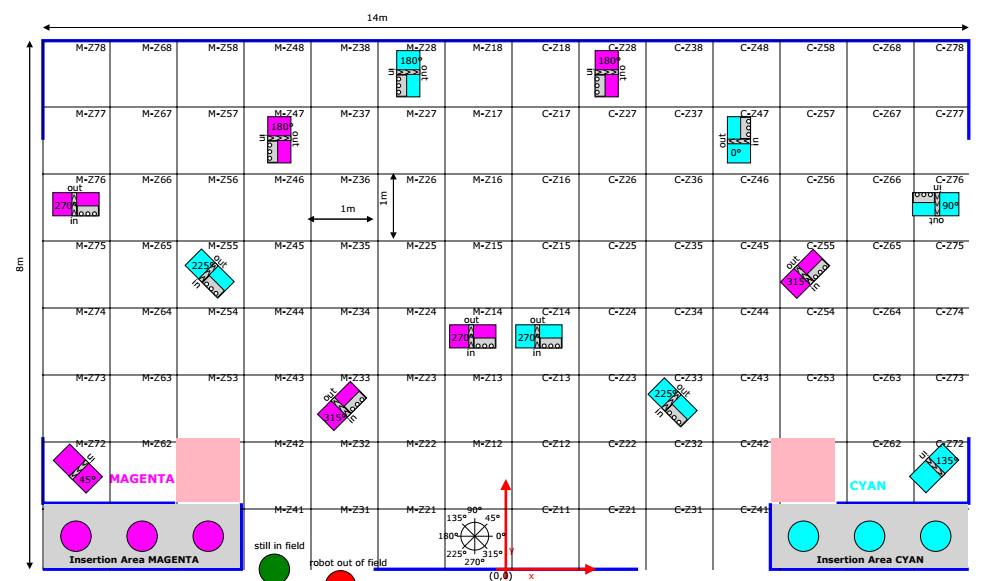
\includegraphics[width=\linewidth]{pic/field.png}
\caption{Field for robocup 2017}
\label{fig:frog}
\end{figure}

\subsection{Difficulties}

Some difficulties have been faced because the Smartbots team has been informed of the new rules during the Robocup. First, it was needed to implement a way to explore field without previous knowledge about the position due to the change in the Rulebook. To face this, a path has been created with some fixed zones in the instruction planer component.  Then, it was necessary to get the zone and the orientation of a detected MPS. This task has not been fulfilled for the Robocup. The last difficulty was to set up the network. There were two configurations, one to test and one to participate to the match.
 

\subsection{Situation in the Robocup}

To conclude, the team could accomplish some actions. First, only one robot was moving for each match because there was no multi-deployment. To do the exploration phase, the robot was going in some fixed positions (landmarks). There was no detection of the zone and the orientation of a MPS however the Alvar tag detection was fully working. The production phase was not implemented and the maintenance phase was not handled. The communication between all component (Refbox Server, Instruction planer, Alvar Tag detection and MPS docking was working and complete. 